\documentclass{beamer}
\usepackage[english]{babel}
\usepackage{amsmath,amssymb,graphicx}

%%%%%%%%%% Start TeXmacs macros
\newcommand{\cdummy}{\cdot}
\newcommand{\mathd}{\mathrm{d}}
\newcommand{\nospace}{}
\newcommand{\point}{.}
\newcommand{\tmfolded}[2]{\trivlist{\item[$\bullet$]\mbox{}#1}}
\newcommand{\tmmathbf}[1]{\ensuremath{\boldsymbol{#1}}}
\newcommand{\tmop}[1]{\ensuremath{\operatorname{#1}}}
\newcommand{\tmunfolded}[2]{\trivlist{\item[$\circ$]\mbox{}#1\\\item[]\mbox{}#2}}
\newenvironment{itemizedot}{\begin{itemize} \renewcommand{\labelitemi}{$\bullet$}\renewcommand{\labelitemii}{$\bullet$}\renewcommand{\labelitemiii}{$\bullet$}\renewcommand{\labelitemiv}{$\bullet$}}{\end{itemize}}
%%%%%%%%%% End TeXmacs macros

\begin{document}

{\slideshow{\begin{frame}
  \
  
  \
  
  \
  
  \
  
  \
  
  \title{计算视觉与模式识别}
  
  \maketitle
\end{frame}

\begin{frame}
  \frametitle{光源}
  
  \
  
  \
  
  出射度
  \begin{eqnarray*}
    E (\tmmathbf{x}) & = & \int_{\Omega} L_e (\tmmathbf{x}, \theta_o,
    \varphi_o) \cos \theta (o) \mathd \omega
  \end{eqnarray*}
\end{frame}

\begin{frame}
  \frametitle{定性辐射学}
  
  {\hspace{4em}}\resizebox{0.7\columnwidth}{!}{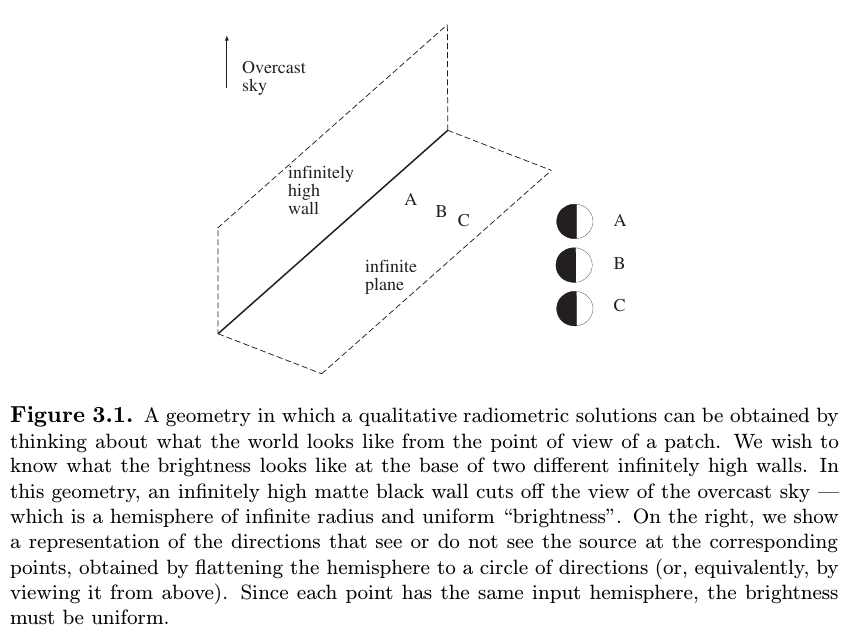
\includegraphics{img/infinitely_high_wall_shaddow.png}}
  
  \ 
\end{frame}

\begin{frame}
  \frametitle{}
  
  {\hspace{4em}}\resizebox{0.7\columnwidth}{!}{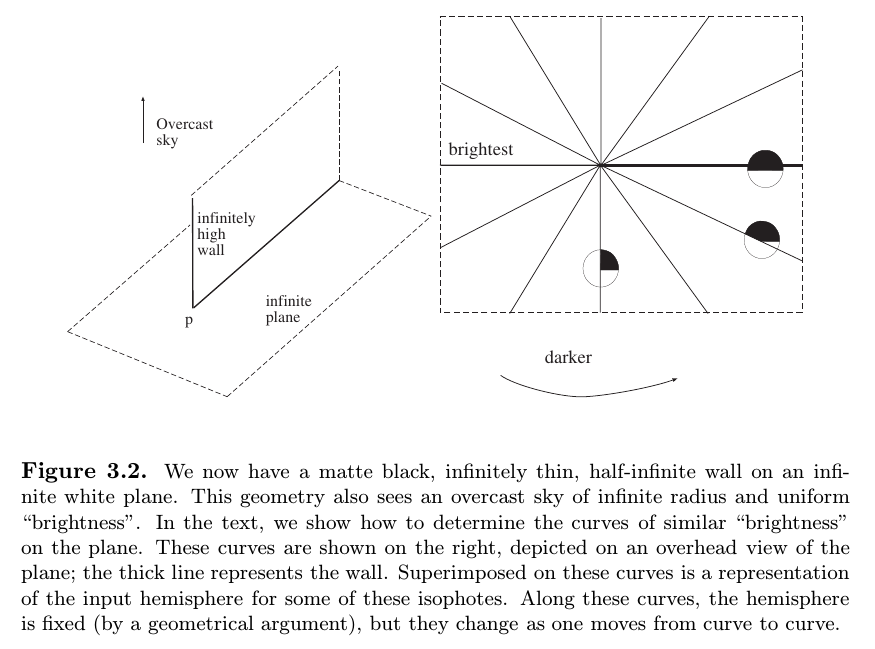
\includegraphics{img/half_infinite_wall.png}}
\end{frame}

\begin{frame}
  \frametitle{光源效果}
  
  {\hspace{5em}}\resizebox{0.6\columnwidth}{!}{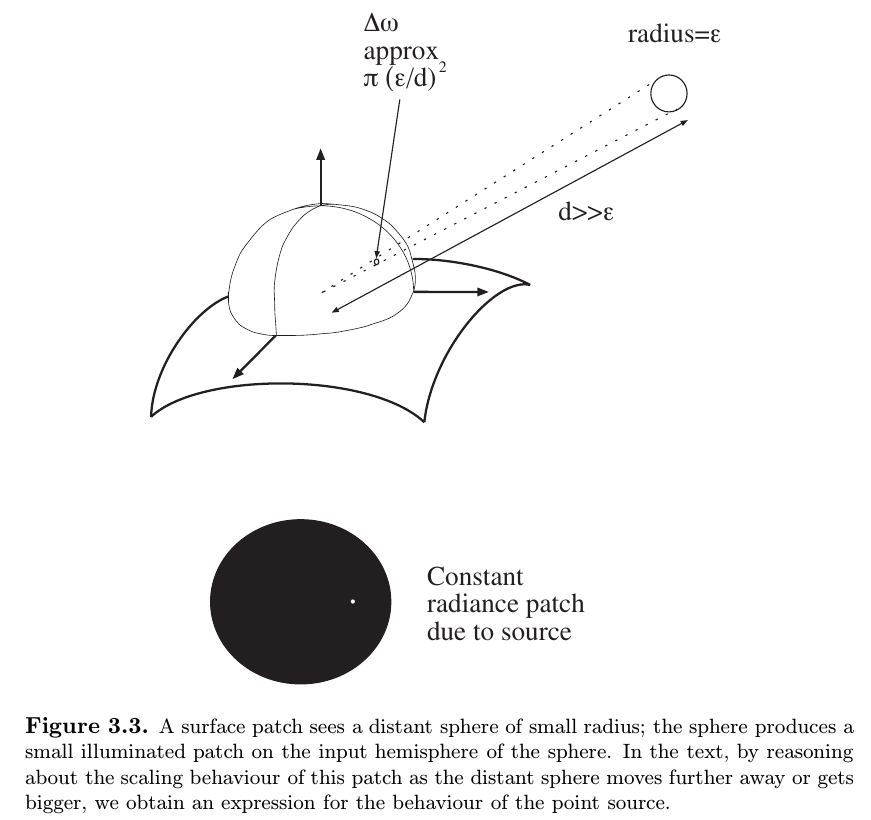
\includegraphics{img/point_sphere_on_surface.png}}
\end{frame}

\begin{frame}
  \frametitle{}
  
  发射度
  \begin{eqnarray*}
    E (x) & = & \int_{\Omega} L_e (x, \theta_o, \varphi_o) \cos \theta_o
    \mathd \omega
  \end{eqnarray*}
  辐射度
  \begin{eqnarray*}
    &  & r \left( \frac{\varepsilon}{r} \right)^2 E \nospace \cos \theta
  \end{eqnarray*}
  
\end{frame}

\begin{frame}
  \frametitle{点光源}
  
  近点光源
  \begin{eqnarray*}
    &  & \rho_d (\tmmathbf{x}) \frac{\tmmathbf{N} (x) \cdummy \tmmathbf{S}
    (\tmmathbf{x})}{r (\tmmathbf{x})^2}
  \end{eqnarray*}
  无穷远点光源
  \begin{eqnarray*}
    \frac{\tmmathbf{N} \cdummy \tmmathbf{S} (\tmmathbf{x})}{r
    (\tmmathbf{x})^2} & = & \frac{\tmmathbf{N} \cdummy (\tmmathbf{S}_0 +
    \Delta \tmmathbf{S} (\tmmathbf{x}))}{(r_0 + r (\tmmathbf{x}))^2}\\
    & \approx & \frac{\tmmathbf{N} \cdummy \tmmathbf{S}_0}{r_0^2}\\
    B (\tmmathbf{x}) & = & \rho_d (\tmmathbf{x}) (\tmmathbf{N} \cdummy
    \tmmathbf{S})
  \end{eqnarray*}
\end{frame}

\begin{frame}
  \frametitle{线光源}
  
  \resizebox{0.9\columnwidth}{!}{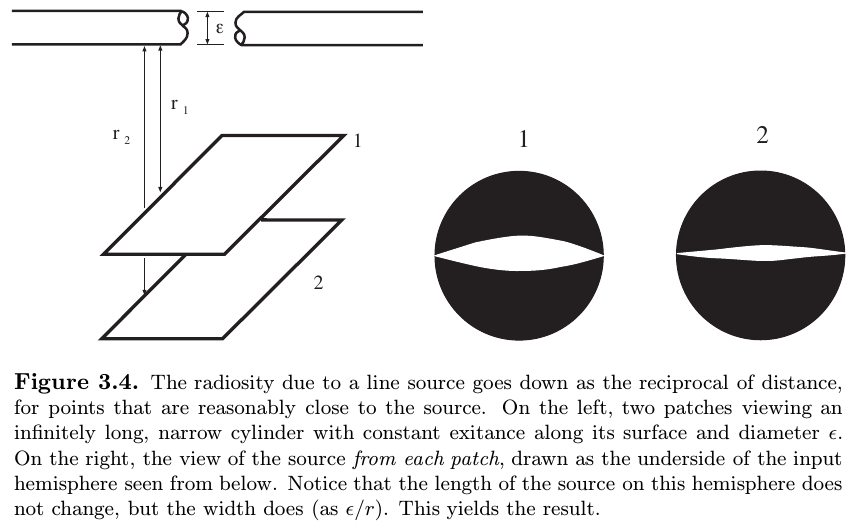
\includegraphics{img/line_source.png}}
\end{frame}

\begin{frame}
  \frametitle{面光源}
  
  {\hspace{7em}}\resizebox{0.5\columnwidth}{!}{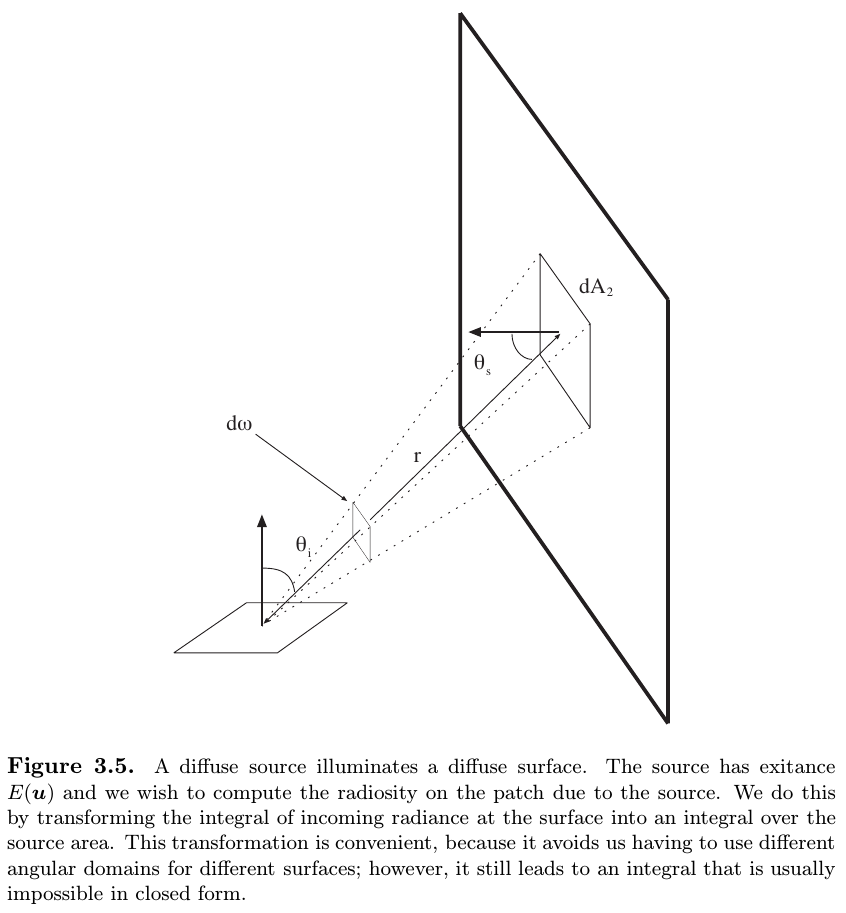
\includegraphics{img/area_source.png}}
\end{frame}

\begin{frame}
  \frametitle{面光源辐射度}
  \begin{eqnarray*}
    B (\tmmathbf{x}) & = & \rho_d (\tmmathbf{x}) \int_{\Omega} L_i
    (\tmmathbf{x}, \tmmathbf{u} \rightarrow \tmmathbf{x}) \cos \theta_i \mathd
    \omega\\
    & = & \rho_d (\tmmathbf{x}) \int_{\Omega} L_e (\tmmathbf{u}, \tmmathbf{u}
    \rightarrow \tmmathbf{x}) \cos \theta_i \mathd \omega\\
    & = & \rho_d (\tmmathbf{x}) \int_{\Omega} \left( \frac{E
    (\tmmathbf{u})}{\pi} \right) \cos \theta_i \mathd \omega\\
    & = & \rho_d (\tmmathbf{x}) \int_{\tmop{Source}} \left( \frac{E
    (\tmmathbf{u})}{\pi} \right) \cos \theta_i \left( \cos \theta_s
    \frac{\mathd A_{\tmmathbf{u}}}{r^2} \right)\\
    & = & \rho_d (\tmmathbf{x}) \int_{\tmop{Source}} \frac{E (\tmmathbf{u})
    \cos \theta_i \cos \theta_s}{\pi r^2} \mathd A_{\tmmathbf{u}}
  \end{eqnarray*}
  \tmfolded{$E (\tmmathbf{u}) = \pi L_e (\tmmathbf{u}, \tmmathbf{u}
  \rightarrow \tmmathbf{x})$}{\begin{eqnarray*}
    E & = & \int_0^{\frac{\pi}{2}} \int_0^{2 \pi} L \cdummy \cos \theta
    \cdummy \sin \theta \mathd \phi \mathd \theta\\
    & = & 2 \pi L \int_0^{\frac{\pi}{2}} \cos \theta \sin \theta \mathd
    \theta\\
    & = & \pi L \int_0^{\frac{\pi}{2}} \sin 2 \theta \mathd \theta\\
    & = & \pi L
  \end{eqnarray*}}
\end{frame}

\begin{frame}
  \frametitle{局部光照模型------点光源}
  
  点光源
  \begin{eqnarray*}
    B (\tmmathbf{x}) & = & \sum_{s \in \{ t|t \rightarrow x \}} B_s
    (\tmmathbf{x})
  \end{eqnarray*}
  无穷远点光源
  \begin{eqnarray*}
    B (\tmmathbf{x}) & = & \sum_{s \in \{ t|t \rightarrow x \}} \rho_d
    (\tmmathbf{x}) \tmmathbf{N} (\tmmathbf{x}) \cdummy \tmmathbf{S}_s
  \end{eqnarray*}
  近点光源
  \begin{eqnarray*}
    B (\tmmathbf{x}) & = & \sum_{s \in \{ t|t \rightarrow x \}} \rho_d
    (\tmmathbf{x}) \frac{\tmmathbf{N} (\tmmathbf{x}) \cdummy \tmmathbf{S}
    (\tmmathbf{x})}{r_s (\tmmathbf{x})^2}
  \end{eqnarray*}
\end{frame}

\begin{frame}
  \frametitle{点光源与阴影}
  
  \qquad\resizebox{.8\columnwidth}{!}{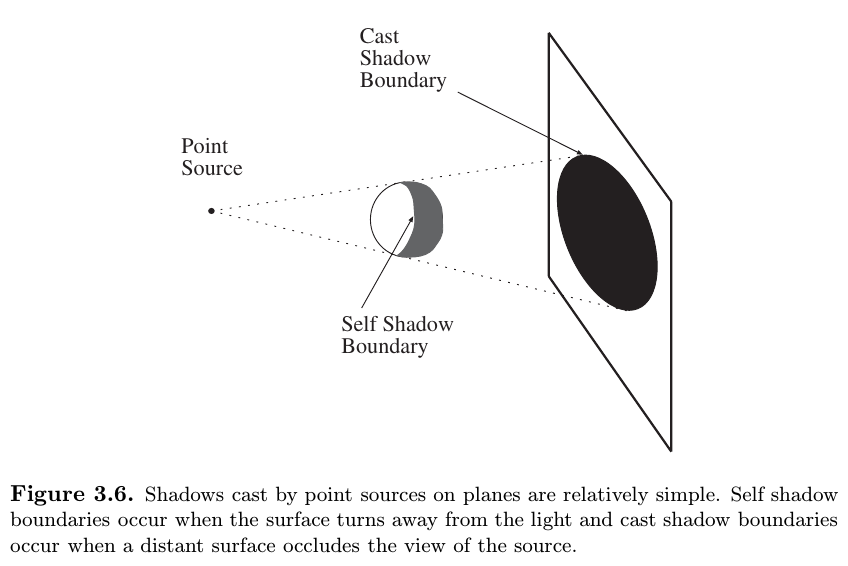
\includegraphics{img/point_source_shadow.png}}
\end{frame}

\begin{frame}
  \frametitle{面光源}
  
  \
  
  
  \begin{eqnarray*}
    B (\tmmathbf{x}) & = & \sum_{s \in \text{all sources}} \left\{
    \int_{\text{visible component of sources s}} \text{Radiosity due to
    source} \right\}\\
    & = & \sum_{s \in \text{all sources}} \int_{\text{visible component of
    sources s}} \text{} \left\{ E (\tmmathbf{u}) \frac{\cos \theta_u \cos
    \theta_s}{\pi r^2} \mathd A_{\tmmathbf{u}} \right\}
  \end{eqnarray*}
\end{frame}

\begin{frame}
  \frametitle{面光源与阴影}
  
  {\hspace{4em}}\resizebox{.6\columnwidth}{!}{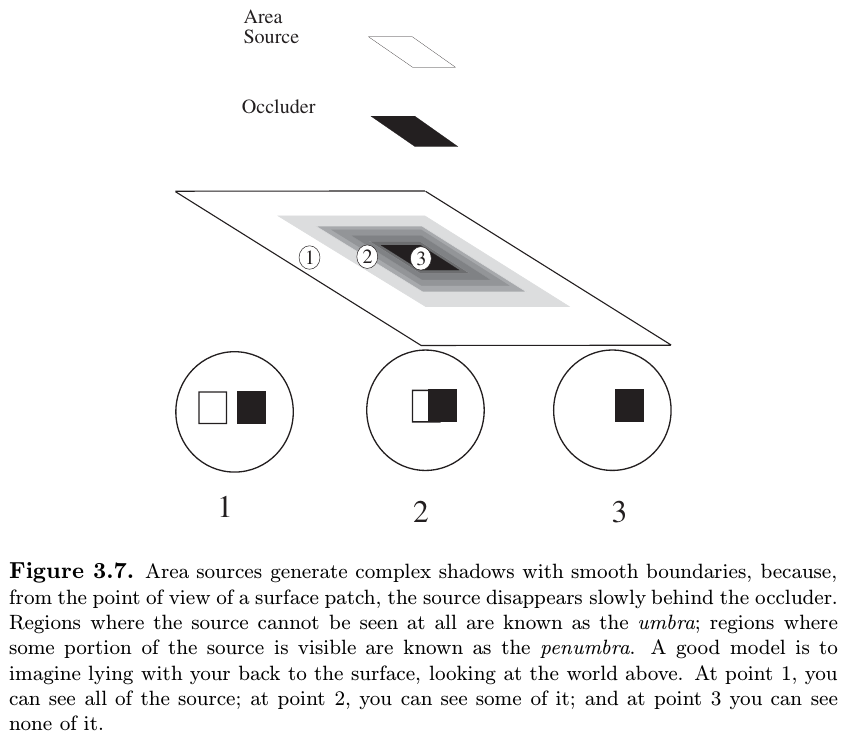
\includegraphics{img/area_source_shadow.png}}
\end{frame}

\begin{frame}
  \frametitle{环境光}
  
  {\hspace{4em}}\resizebox{0.6\columnwidth}{!}{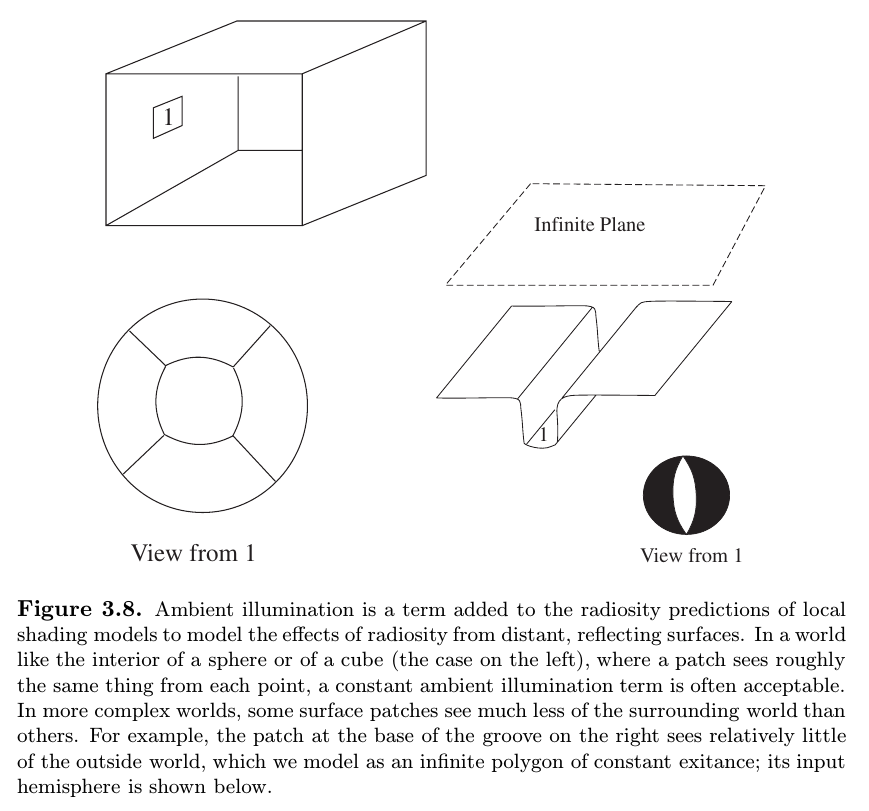
\includegraphics{img/ambient_illumination.png}}
\end{frame}

\begin{frame}
  \frametitle{表面反射}
  
  \resizebox{1\columnwidth}{!}{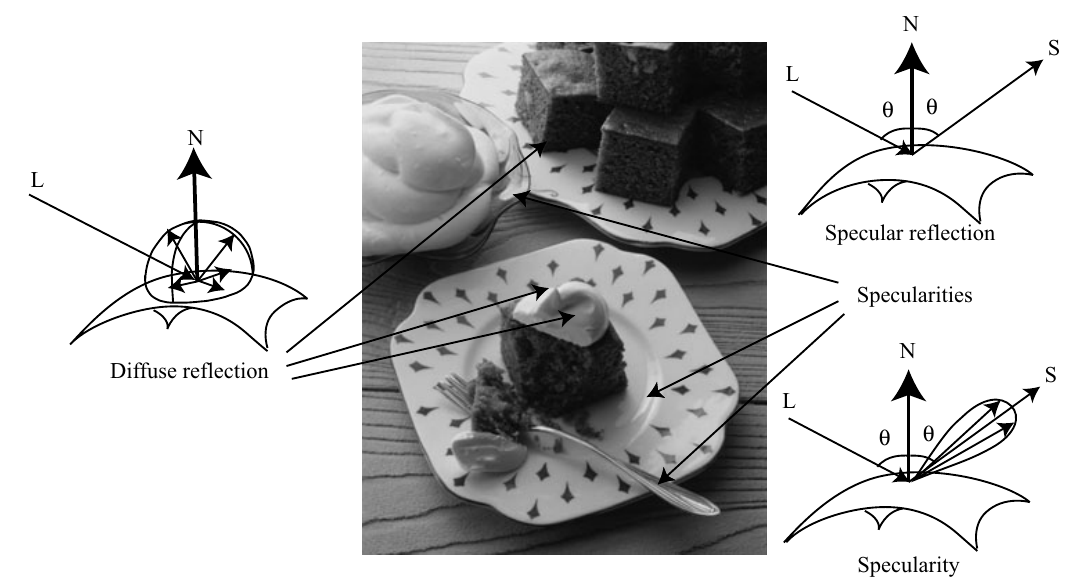
\includegraphics{img/surface_reflection.png}}
\end{frame}

\begin{frame}
  \frametitle{朗伯与镜面反射模型}
  
  \
  
  
  \[ \begin{array}{lllllll}
       I (\tmmathbf{x}) & = & \rho (\tmmathbf{x}) (\tmmathbf{N} \cdummy
       \tmmathbf{S}) \tmop{Vis} (\tmmathbf{S}, \tmmathbf{x}) & + & \rho
       (\tmmathbf{x}) A & + & M\\
       \tmop{Image} &  & \tmop{Diffuse} & + & \tmop{Ambient} & + &
       \tmop{Specular} (\tmop{mirror} - \tmop{like})\\
       \tmop{intensity} &  & \tmop{term} &  & \tmop{term} &  & \tmop{term}
     \end{array} \]
\end{frame}

\begin{frame}
  \frametitle{辐射标定}
  
  
  \begin{eqnarray*}
    I^{(k)}_{i \nospace j} & = & f (E_{i \nospace j} \Delta t_k)\\
    \log \nospace g (I_{i \nospace j}^{(k)}) & = & \log \nospace E_{i \nospace
    j} + \log \Delta t_k
  \end{eqnarray*}
  估计$g = f^{- 1}$, 损失函数:
  \begin{eqnarray*}
    \sum_{i, j, k} (\log \nospace g (I_{i \nospace j}^{(k)}) - (\log \nospace
    E_{i \nospace j} + \log \Delta t_k))^2 + \text{smoothness penalty on $g$}
    &  & 
  \end{eqnarray*}
  估计$E_{i \nospace j}$
  \begin{eqnarray*}
    \sum_k w (I_{i \nospace j}) (I^{(k)}_{i \nospace j} - f (E_{i \nospace j}
    \Delta t_k))^2 &  & 
  \end{eqnarray*}
\end{frame}

\begin{frame}
  \frametitle{辐射标定示例}
  
  \resizebox{1\columnwidth}{!}{\includegraphics{img/calibrate_radiometric
  .png}}
\end{frame}

\begin{frame}
  \frametitle{镜面反射形状}
  
  \resizebox{1\columnwidth}{!}{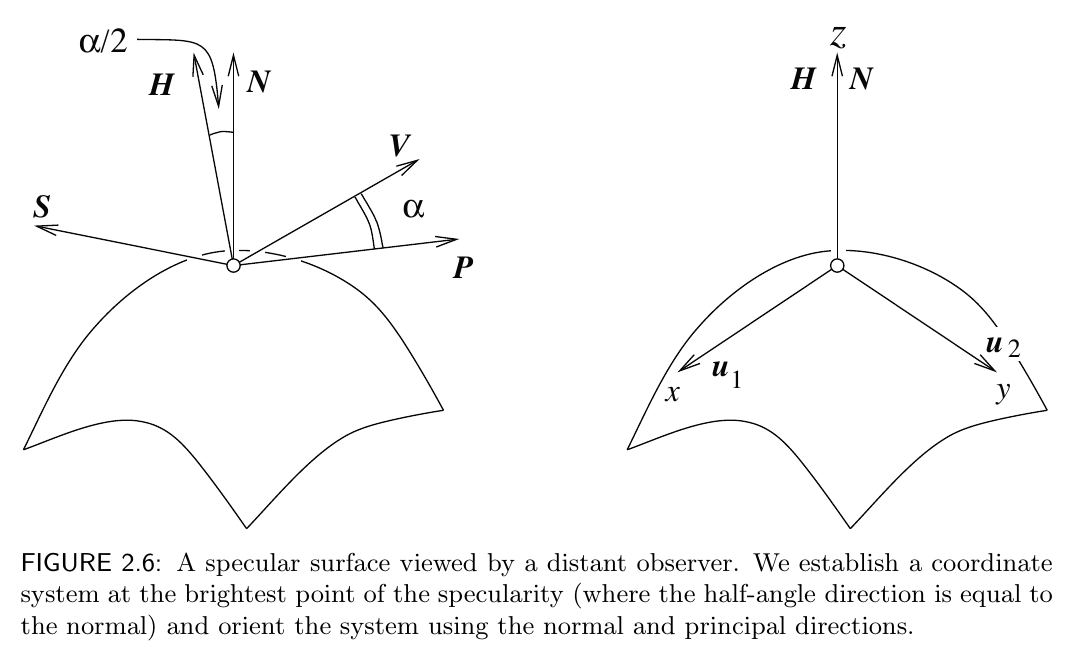
\includegraphics{img/specular_surface_coordinate.png}}
\end{frame}

\begin{frame}
  \frametitle{镜面反射的边界}
  
  
  \begin{eqnarray*}
    \tmmathbf{V} \cdummy \tmmathbf{P} & \geqslant & 1 - \varepsilon\\
    1 - \varepsilon & = & \tmmathbf{V} \cdummy \tmmathbf{P}\\
    & = & 2 \frac{(\tmmathbf{H} \point \tmmathbf{N})^2}{(\tmmathbf{H} \cdummy
    \tmmathbf{H})} - 1
  \end{eqnarray*}
  \begin{eqnarray*}
    z & = & - \frac{1}{2} (\kappa_1 x^2 + \kappa_2 y^2)\\
    \tmmathbf{N} & = & (1 + \kappa^2_1 x^2 + \kappa^2_2 y^2)^{- \frac{1}{2}}
    \left(\begin{array}{ccc}
      \kappa_1 x & \kappa_2 y & 1
    \end{array}\right)^T
  \end{eqnarray*}
  \begin{eqnarray*}
    \kappa^2_1 x^2 + \kappa_2^2 y^2 & = & \zeta
  \end{eqnarray*}
\end{frame}

\begin{frame}
  \frametitle{镜面反射的移动}
  
  \resizebox{1\columnwidth}{!}{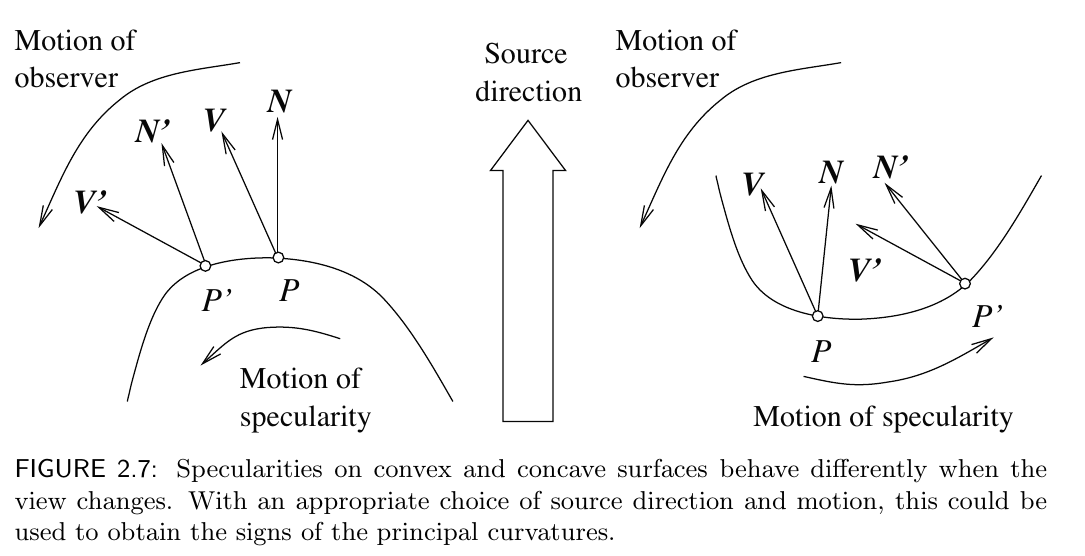
\includegraphics{img/specularities_convex_concave.png}}
\end{frame}

\begin{frame}
  \frametitle{}
  
  $\tmmathbf{S}$不变 :
  \begin{eqnarray*}
    \tmmathbf{V} & = & 2 (\tmmathbf{S} \cdummy \tmmathbf{N})
    \tmmathbf{N}-\tmmathbf{S}\\
    \delta \tmmathbf{V} & = & 2 (\tmmathbf{S} \cdummy (\tmmathbf{N}+ \delta
    \tmmathbf{N})) (\tmmathbf{N}+ \delta \tmmathbf{N})
    -\tmmathbf{S}-\tmmathbf{V}\\
    & = & 2 (\tmmathbf{S} \cdummy \delta \tmmathbf{N}) \tmmathbf{N}+ 2
    (\tmmathbf{S} \cdummy \tmmathbf{N}) \delta \tmmathbf{N}+ 2 (\tmmathbf{S}
    \cdummy \mathd \tmmathbf{N}) \mathd \tmmathbf{N}\\
    \mathd \tmmathbf{V} & = & 2 (\tmmathbf{S} \cdummy \mathd \tmmathbf{N})
    \tmmathbf{N}+ 2 (\tmmathbf{S} \cdummy \tmmathbf{N}) \mathd \tmmathbf{N}+ 2
    (\tmmathbf{S} \cdummy \mathd \tmmathbf{N}) \mathd \tmmathbf{N}
  \end{eqnarray*}
  得
  \begin{eqnarray*}
    \mathd \tmmathbf{V} \cdummy \mathd \tmmathbf{r} & = & 2 (\tmmathbf{S}
    \cdummy \tmmathbf{N}) \mathd \tmmathbf{N} \cdummy \mathd \tmmathbf{r}
    \hspace{5em} \mathd \tmmathbf{r}=\tmmathbf{r}_s \mathd s
  \end{eqnarray*}
\end{frame}

\begin{frame}
  \frametitle{亮度与照度推理}
  
  相机响应
  \begin{eqnarray*}
    C (\tmmathbf{x}) & = & k_c I (\tmmathbf{x}) \rho (\tmmathbf{x})\\
    \log \nospace C (\tmmathbf{x}) & = & \log \nospace k_c + \log \nospace I
    (\tmmathbf{x}) + \log \nospace \rho (\tmmathbf{x})
  \end{eqnarray*}
  \tmunfolded{$\rho
  (\tmmathbf{x})$:反射率}{同一物体基本不变,不同物体边界处有突变}
  
  \tmunfolded{$I (\tmmathbf{x})$:光照}{变化缓慢}
  
  \
  
  \
  
  \ 
\end{frame}

\begin{frame}
  \frametitle{亮度算法示例}
  
  {\hspace{7em}}\resizebox{0.5\columnwidth}{!}{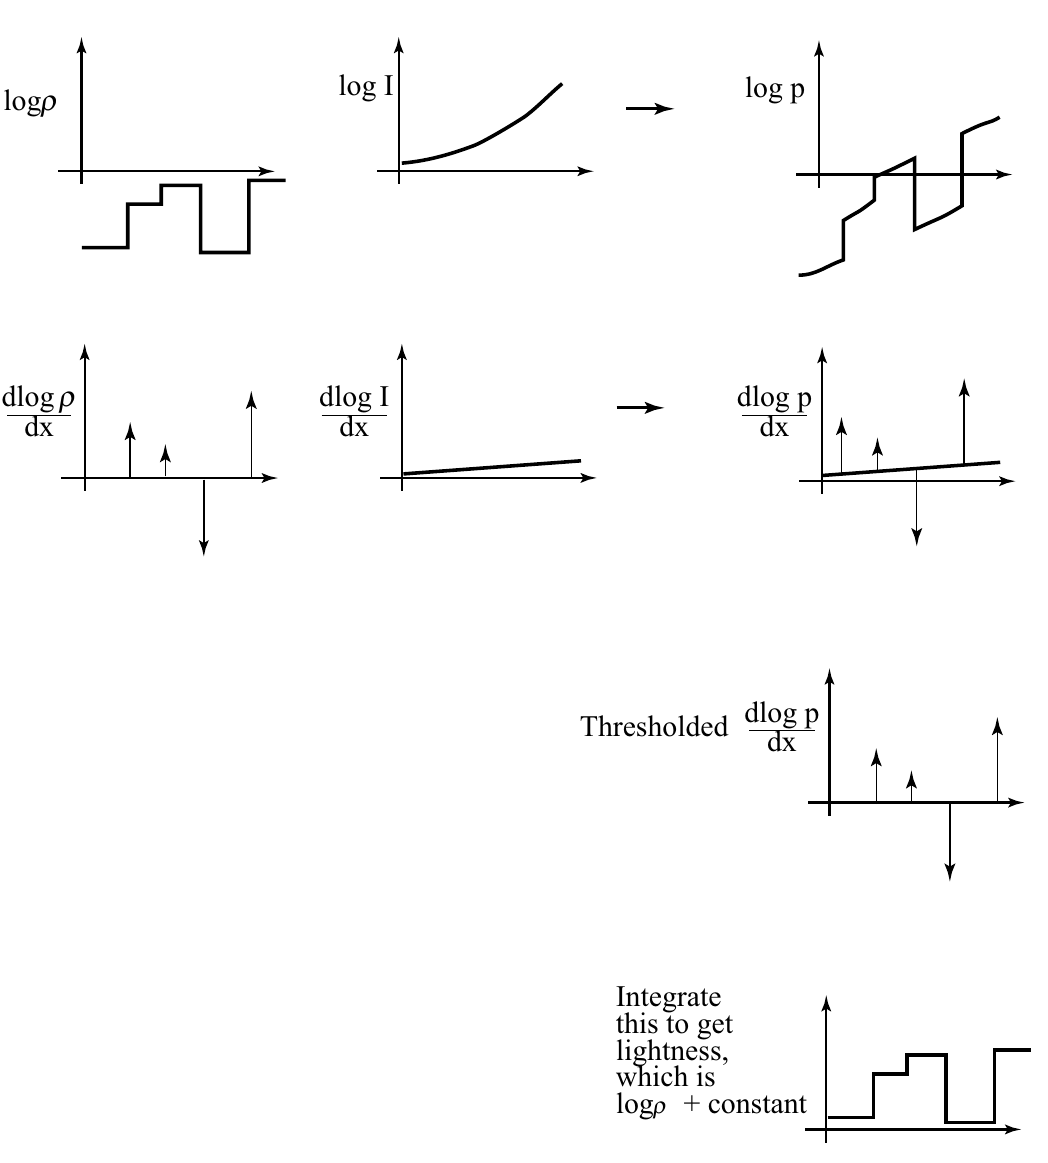
\includegraphics{img/inferring_lightness_and_illumination.png}}
\end{frame}

\begin{frame}
  \frametitle{估计反射率}
  
  
  \begin{itemizedot}
    \item 计算阈值化梯度
    
    \item 积分
  \end{itemizedot}
  
  
  或
  
  
  \begin{itemizedot}
    \item 计算阈值化梯度$\tmmathbf{p}, \tmmathbf{q}$
    
    \item 最小化
    \begin{eqnarray*}
      | \mathcal{M}_x \tmmathbf{l}-\tmmathbf{p} |^2 + | \mathcal{M}_y
      \tmmathbf{l}-\tmmathbf{q} |^2 &  & 
    \end{eqnarray*}
  \end{itemizedot}
  
\end{frame}

\begin{frame}
  \frametitle{光度立体法}
  
  \resizebox{1\columnwidth}{!}{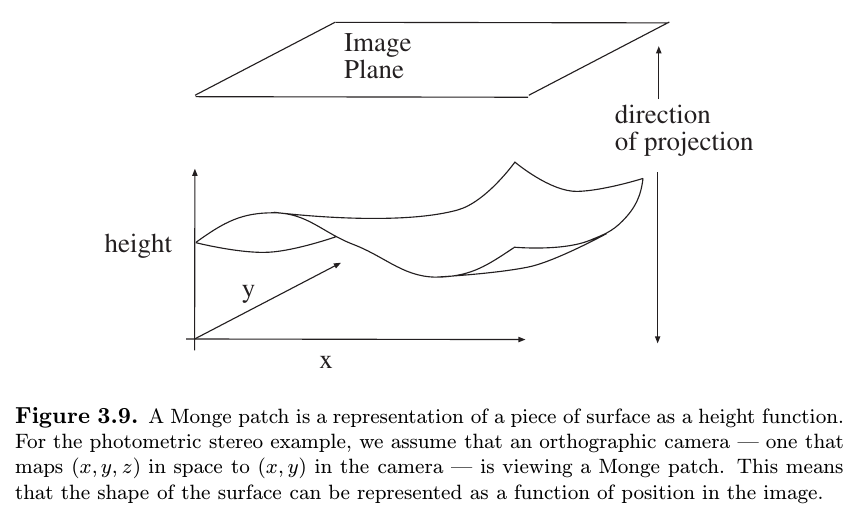
\includegraphics{img/monge_patch.png}}
\end{frame}

\begin{frame}
  \frametitle{}
  
  {\hspace{3em}}\resizebox{0.8\columnwidth}{!}{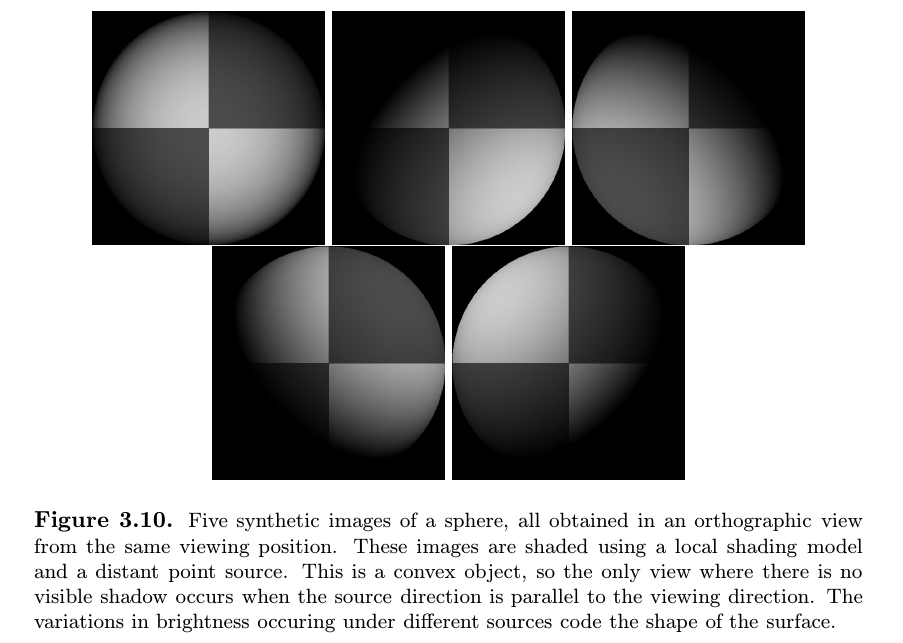
\includegraphics{img/shading_sphere.png}}
\end{frame}

\begin{frame}
  \frametitle{图像与法向量}
  \begin{eqnarray*}
    B (x) & = & \rho (x) \tmmathbf{N} (x) \cdummy \tmmathbf{S}_1\\
    I (x, y) & = & k \nospace B (\tmmathbf{x})\\
    & = & k \nospace B (x, y)\\
    & = & k \rho (x, y) \tmmathbf{N} (x, y) \cdummy \tmmathbf{S}_1\\
    & = & \tmmathbf{g} (x, y) \cdummy \tmmathbf{V}_1\\
    g (x, y) & = & \rho (x, y) \tmmathbf{N} (x, y)\\
    \tmmathbf{V}_1 & = & k\tmmathbf{S}_1
  \end{eqnarray*}
  
\end{frame}

\begin{frame}
  \frametitle{法向量计算}
  \begin{eqnarray*}
    \tmmathbf{i} (x, y) & = & \left(\begin{array}{cccc}
      I_1 (x, y) & I_2 (x, y) & \cdots & I_n (x, y)
    \end{array}\right)^T\\
    & = & \mathcal{V}\tmmathbf{g} (x, y)\\
    \mathcal{V} & = & \left(\begin{array}{c}
      \tmmathbf{V}^T_1\\
      \tmmathbf{V}^T_2\\
      \vdots\\
      \tmmathbf{V}^T_n
    \end{array}\right)
  \end{eqnarray*}
  得
  \begin{eqnarray*}
    \tmmathbf{N} (x, y) & = & \frac{\tmmathbf{g} (x, y)}{| \tmmathbf{g} (x, y)
    |}\\
    | \tmmathbf{g} (x, y) | & = & \rho (x, y)
  \end{eqnarray*}
\end{frame}

\begin{frame}
  \frametitle{法向量场}
  
  \resizebox{0.9\columnwidth}{!}{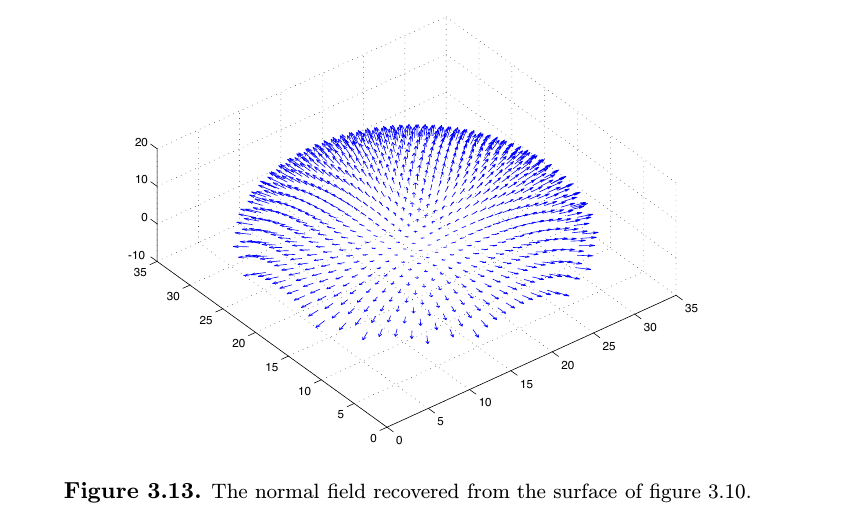
\includegraphics{img/normal_field_sphere.png}}
\end{frame}

\begin{frame}
  \frametitle{从法向量获取形状}
  \begin{eqnarray*}
    \tmmathbf{N} (x, y) & = & \left( 1 + \frac{\partial f^2}{\partial x} +
    \frac{\partial f^2}{\partial y} \right)^{- \frac{1}{2}}
    \left(\begin{array}{ccc}
      \frac{\partial f}{\partial x} & \frac{\partial f}{\partial y} & 1
    \end{array}\right)^T\\
    f (x, y) & = & \oint_C \left(\begin{array}{cc}
      \frac{\partial f}{\partial x} & \frac{\partial f}{\partial y}
    \end{array}\right)^T \cdummy \mathd \tmmathbf{l}+ c
  \end{eqnarray*}
  $l : (0, 0) \rightarrow (0, v) \rightarrow (u, v)$
  \begin{eqnarray*}
    f (u, v) & = & \int_o^v \frac{\partial f}{\partial y}
    \left(\begin{array}{cc}
      0 & y
    \end{array}\right) \mathd y + \int_o^u \frac{\partial f}{\partial x}
    \left(\begin{array}{cc}
      x & v
    \end{array}\right) \mathd x + c
  \end{eqnarray*}
\end{frame}

\begin{frame}
  \frametitle{法向量场到高度场}
  
  \resizebox{0.9\columnwidth}{!}{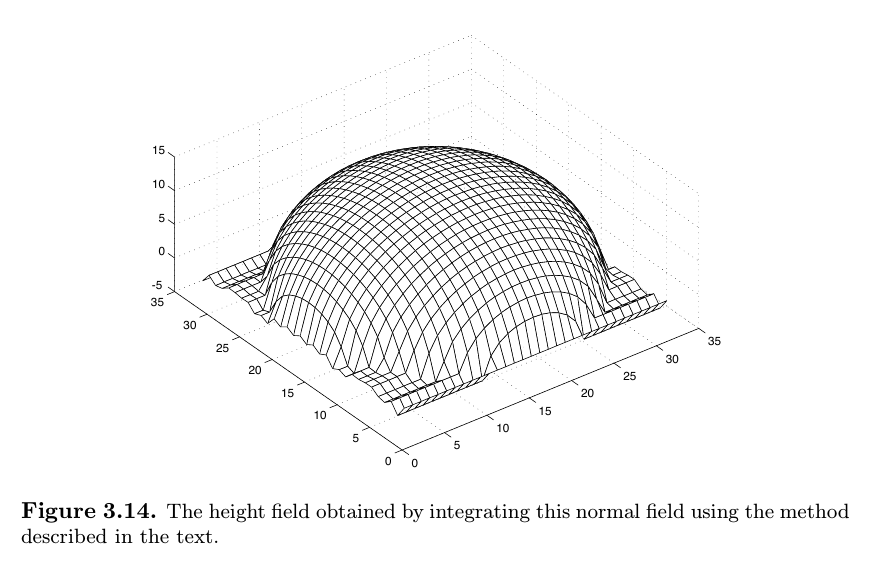
\includegraphics{img/height_field.png}}
\end{frame}

\begin{frame}
  \frametitle{互反射}
  
  \qquad\resizebox{0.8\columnwidth}{!}{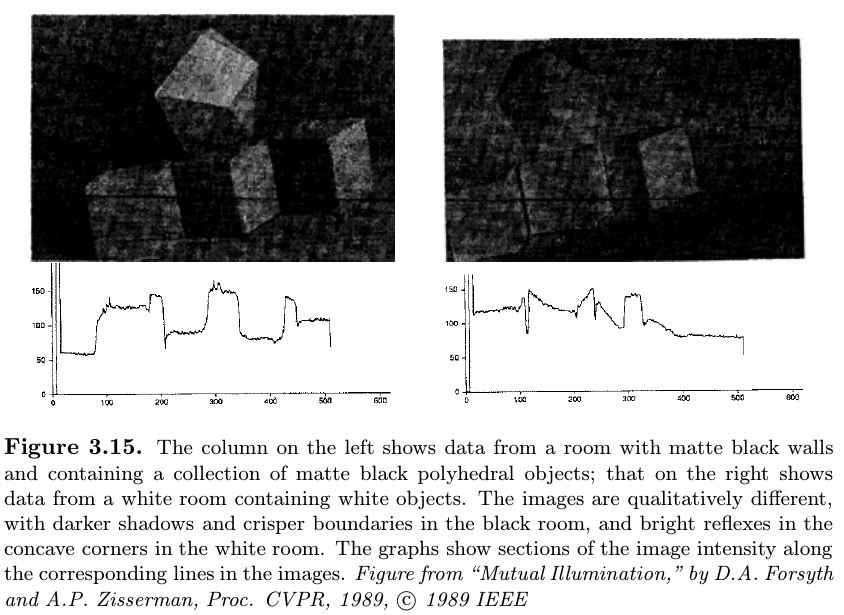
\includegraphics{img/interreflection.png}}
\end{frame}

\begin{frame}
  \frametitle{互反射模型}
  
  \quad\resizebox{0.9\columnwidth}{!}{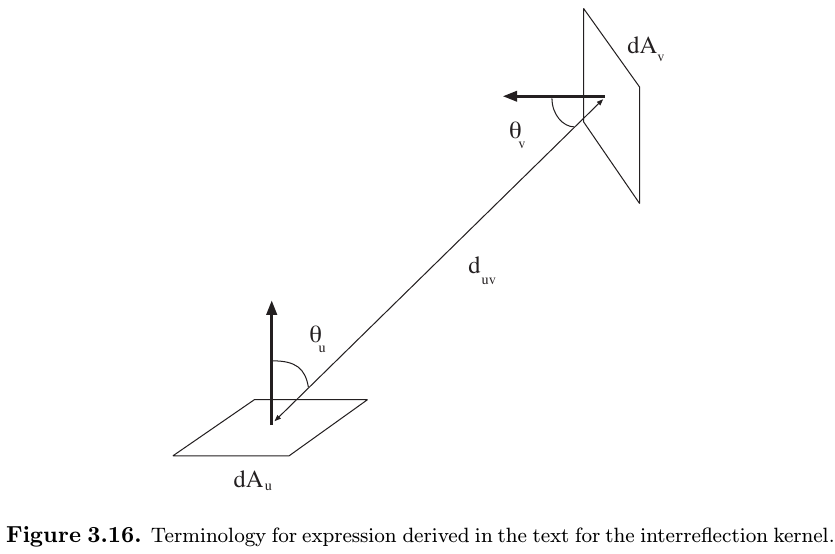
\includegraphics{img/interreflection_kernel_terminology.png}}
\end{frame}

\begin{frame}
  \frametitle{计算出射度}
  \begin{eqnarray*}
    B (\tmmathbf{u}) & = & E (\tmmathbf{u}) + B_{\tmop{incoming}}
    (\tmmathbf{u})\\
    B_{\tmop{incoming}} (\tmmathbf{u}) & = & \rho_d (\tmmathbf{u})
    \int_{\tmop{world}} \tmop{visible} (\tmmathbf{u}, \tmmathbf{v}) B
    (\tmmathbf{v}) \frac{\cos \theta_u \cos \theta_v}{\pi d^2_{u \nospace v}}
    \mathd A_{\tmmathbf{v}}\\
    & = & \rho_d (\tmmathbf{u}) \int_{\tmop{world}} \tmop{visible}
    (\tmmathbf{u}, \tmmathbf{v}) B (\tmmathbf{v}) K (\tmmathbf{u},
    \tmmathbf{v}) \mathd A_{\tmmathbf{v}}\\
    B_{j \rightarrow i} (\tmmathbf{x}) & = & \rho_d (x) \int_{\tmop{patch} j}
    \tmop{visible} (\tmmathbf{x}, \tmmathbf{v}) K (\tmmathbf{x}, \tmmathbf{v})
    \mathd A_{\tmmathbf{v}} B_j\\
    \bar{B}_{j \rightarrow i} & = & \frac{1}{A_i} \int_{\tmop{path} i} \rho_d
    (x) \int_{\tmop{patch} j} \tmop{visible} (\tmmathbf{x}, \tmmathbf{v}) K
    (\tmmathbf{x}, \tmmathbf{v}) \mathd A_{\tmmathbf{v}} \mathd
    A_{\tmmathbf{x}} B_j
  \end{eqnarray*}
\end{frame}

\begin{frame}
  \frametitle{}
  \begin{eqnarray*}
    B_i & = & E_i + \sum_{\tmop{all} j} B_{\text{average incoming at $i$ from
    $j$}}\\
    & = & E_i + \sum_{\tmop{all} j} K_{i \nospace j} B_j
  \end{eqnarray*}
  where
  \begin{eqnarray*}
    K_{i \nospace j} & = & \frac{1}{A_i} \int_{\tmop{path} i} \rho_d (x)
    \int_{\tmop{patch} j} \tmop{visible} (\tmmathbf{x}, \tmmathbf{v}) K
    (\tmmathbf{x}, \tmmathbf{v}) \mathd A_{\tmmathbf{v}} \mathd
    A_{\tmmathbf{x}}
  \end{eqnarray*}
\end{frame}}}

\end{document}
